\documentclass[12pt]{article}
%\usepackage{kpfonts}
\usepackage{graphicx}
\usepackage{float}
\usepackage{algorithm}
\usepackage{amsmath}
\usepackage[noend]{algpseudocode}
\usepackage{amssymb}
\usepackage{bm}

\makeatletter
\def\BState{\State\hskip-\ALG@thistlm}
\makeatother

%\algnewcommand\algorithmicforeach{\textbf{for each:}}
%\algnewcommand\ForEach{\item[ \algorithmicforeach]}

\algnewcommand\algorithmicforeach{\textbf{for each}}
\algdef{S}[FOR]{ForEach}[1]{\algorithmicforeach\ #1\ \algorithmicdo}

\DeclareMathOperator*{\argmin}{\arg\!\min}
\DeclareMathOperator*{\argmax}{\arg\!\max}

\begin{document}

\begin{center}

Topic Extraction Pipeline Outline


\end{center}

\section{Problem Definition}
Popular topic extraction methods used today are frequency and engineered-features based. We propose a data-driven method to automatically extract topics from text based on semantic relationships. In this work, we describe the derivation of this method, as well as research its applications.

\section{Dataset and Data Preprocessing}

We use the GloVe word embedding dataset for mapping strings to vectors.
We remove non-alphabet characters, single character words, and to make all strings lower-case. We also normalize embeddings, so computation of the cosine distance is reduced to dot product operations.\\


\subsection{Representing Words as Embeddings}
 Embedding vectors are an efficient way to represent a vocabulary in a compact, non-sparse, continuous way. One attractive property of word embeddings is that words with similar meaning lie close to each other on embedding space, effectively capturing semantic relationships. We use the GloVe embedding dataset to map text to an embedding representation.
Due to memory limitations, we work with embeddings of size 50.

\section{Keywords, Local Topics, and Topics}
In order to extract \textbf{topics} i.e. high-level ideas that encapsulate the main points found in text, we consider a strict subset of the input text.
The reasoning behind this search approach is that we should only consider words that are relevant and informative while avoiding common and non-informative terms.
Once extracted, these relevant terms may lead us directly into a set of implicit topics found in any input text. The implicitness of the topics is a big aspect for
our keyword extraction approach. Given any input text, we wish to correctly infer the topics the text is \textit{about}, even though these topics are not
explicitly specified.
We search for \textbf{keywords} that will lead us to topics. We define a keyword as a relevant and informative word found in a sentence. Thus, our goal
is to first extract keywords from a set of sentences i.e. a paragraph or section in a research paper, and from those keywords infer a \textbf{local topic}.
We define a local topic as the main idea behind a related set of sentences e.g. a paragraph or section in a research paper. Having broken down an input text
i.e. extracted a set of local topics, we infer a set of topics that hopefully correctly encapsulate the main ideas behind the text.
\section{Advantages over LDA and Frequency Based Keyword Extractors}
LDA is the standard method used for topic extraction. It is reliable but nonetheless faces important shortcomings. Some known limitation of LDA are:
\begin{itemize}
\item Robust with short text. No parameter estimation for latent topic estimation.
\item No need for fixed K (the number of topics is not fixed and need not be known ahead of time)
\item LDA has Uncorrelated topics (Dirichlet topic distribution cannot capture correlations)
\item LDA outputs topics as a mixture of words, our method outputs a set of high-level terms infered to be topics
\item LDA topics, being composed of mixtures of words, can have terms be part of more than one topic
\item Not scalable: LDA is not scalable to large amounts of text. Our method works in a localized manner, extracting low level information from
chunks of the input text first i.e. extract keywords and local topics, then takes a bottom-up approach infering high level information i.e. topics.
This allows for high scalability and is easily paralellizable
\end{itemize}


\subsection{Advantages and Disadvantages over Frequency Based Keyword Extractors}
Some advantages include:
\begin{itemize}
\item Robust to short text: Frequency based keyword extractors assign importance or weight to terms based on frequency If a term is not frequently
occurring, conventional keyword extractors will assign the same importance to relevant words as to common and irrelevant terms. Our method completely
ignores frequency and these handcrafted features and makes decisions based on semantic relations of the terms in euclidean space.
\item No n-gram or minimum frequency specification is required.
\item Conventional methods rely on engineered features such as whether or not the term was found in the title. Our method ignores such features and
evaluates words solely on semantic relations.
Some disadvanteges include:
\item Our keyword extraction method is more time consuming than frequency based approaches, since dot product operations are at the core of our method. This
may be alleviated via GPU computations of vector operations.
\item Our method relies on a learned word embedding vocabulary. This means we rely on a set of embeddings that reflect semantic properties accurately on
Euclidean space.
\end{itemize}



\section{Keyword Extraction: Finding Relevant Words Within Text}
In order to extract a set of topics from our text data, we must consider only a small subset of the entire text. This means we must find a set of
relevant, meaningful and informative words which we can infer a $\textbf{topic}$ from. In order to find these meaningful words, we must search in
input document space based on some search criteria. First we consider searching for words considering their \textit{within-sentence sum of cosine similarites}.
This search criterion is motivated by the assumption that \textbf{rare} words are informative. The term \textit{rare} in this context means a word
that has low cosine similarity with all other words in the sentence. Consider the scenario of a sentence defining a term. The whole sentence can be
thought of as a collection of words used to define a single word. In this extreme case, the entire sentence i.e. the definition can be compressed by a
single word, the word being defined. Similarly, terms that provide high information to the reader are usually described by a larger set of words.
Thus, we consider these \textit{rare} terms to be highly informative and relevant to the reader and overall information content found in the text.

A second search criterion we incorporate in our keyword search is to have the sum of cosine similarites between all keywords, one for each sentence,
be as high as possible. This choice is justified by the assumption that a paragraph or section of a text will carry around a \textit{local topic}
throughout its sentences. In summary, our two search criteria are as follows:

\begin{itemize}
  \item Minimize within-sentence sum of cosine similarities: Find the most \textit{different} word in a sentence. This word is assumed to be highly informative
  \item Maximize over-sentences sum of cosine similarities: Find the set of words, one word for each sentence, such that the sum of cosine similarites between these words is maximal. This is assumed to be a sort of \textit{topic} found within the input text.
\end{itemize}
In the sections below, we describe the search criteria we used for keyword extraction with further detail.

\subsection{Search Criterion 1: Minimizing Within-Sentence Sum of Cosine Similarities}
One simple method is to extract all words that minimize their sum of cosine distance with all other words within their sentence where they appear. A well known property of word embeddings learned through learning a language model is that they encapsulate semantic relations in embedding space. \\

The reasoning behind this search criterion is that words which are not similar to the other words within a sentence may be more informative and should be considered. In algorithm 1, by the matrix multiplication of a sentence $s$ with its transpose $s^T$ computes the cosine similarity matrix $C$. The column-wise sum gives us a sum of cosine similarities for each term in the sentence. Finding the term that minimizes this similarity measure is equvalent to finding the term that maximizes the sum of cosine distances. By minimizing the cosine similarity between terms, we hope to find words that are relevant and signficant.

\begin{algorithm}[H]
\caption{Search Criterion 1}\label{euclid}
\begin{algorithmic}[1]
\Procedure{SearchCriterion1}{S}
\State $W \gets \emptyset $
\ForEach {$s \in S$}
\State $ C \gets s^ T \cdot s$
\State $ W \cup \argmin\limits_{i} \sum\limits_{j} C_{i,j}$
\State
\EndFor
\State \Return $W$
\EndProcedure
\end{algorithmic}
\end{algorithm}

Consider an input set of sentences $\bm{S} = \{s_1, ..., s_n\}$, where $n = |\bm{S}|$. Each sentence $s_i$ is comprised of a set of embeddings as $s_i = \{e^{i}_{1}, ..., e^{i}_{|s_i|}\}$,  $e^{i}_{k} \in \mathbb{R}^{p}$. For each sentence $s_i$, we compute its cosine similarity matrix as

\[\bm{C_i} = \begin{bmatrix}
         e^{i}_{1} \\
         \vdots \\
         e^{i}_{|s_i|} \\
        \end{bmatrix} \times  \begin{bmatrix}
         e^{i}_{1} \\
         \vdots \\
         e^{i}_{|s_i|} \\
        \end{bmatrix}^{T}\]

We then compute, for each embedding $e^{i}_{j}, j = 1,...,|s_i|$, its \textit{within-sentence} sum of cosine similarities as
\[ c^{i}_{j} = \sum^{|s_i|}_{k=1} \bm{C_{i{_{(k,j)}}}}\]
We denote the $i$th sentence's list of \textit{cosine similarities sums} as
\[\bm{\vec{c_i}} = \{ c^{i}_{1}, ...,  c^{i}_{|s_i|}\}\]


\subsection{Search Criterion 2: Maximizing Over-Paragraph Sum of Cosine Similarities}
Another search criterion we consider is to select keywords by maximizing their $\textit{over-paragraph}$ sum of cosine similarities. This means that the set of keywords we end up selecting, one word per sentence, would result in a \textbf{maximal} sum of cosine similarities.

\begin{algorithm}[H]
\caption{Search Criterion 2 (Brute Approach)}\label{euclid}
\begin{algorithmic}[1]
\Procedure{SearchCriterion2}{S}
\State $i^{*} \gets 0 $
\State $c^{*} \gets -\infty$
\State $E \gets S_{1} \times \dots \times S_{|S|}$
\ForEach{$E_i \in E$}
\State$c \gets  \sum\limits_{j} E_{i}^{j}$
\If {$c > c^{*}$}
\State $c^{*} \gets c$
\State$ i^{*} \gets i$

\EndIf
\EndFor
\State \Return $E_{i^{*}}$
\EndProcedure
\end{algorithmic}
\end{algorithm}

The algorithm above tries all possible combinations of words, one word per sentence, and returns a reference to the set of words that maximized its sum of cosine similarities. This means we extract the set of words, one per sentence,  that are the closest in meaning within an input text. Of course, this method would always select words that are the same, or really close in meaning, but won't enforce any condition of how relevant the words are i.e. how truly the output words are \textit{keywords}.


From this point on in the text, we will refer to these search criteria as \textit{criterion 1 and criterion 2}, respectively.



\begin{figure}[H]
\centering
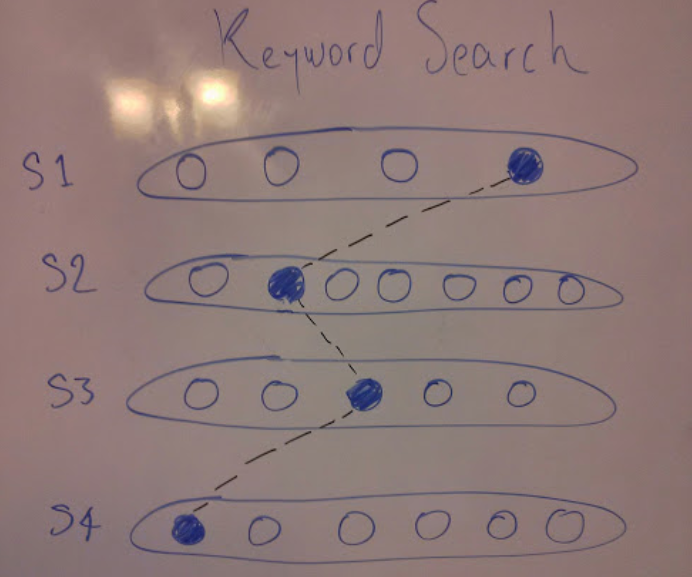
\includegraphics[height=2in, width=4in]{Images/KeywordSearch.png}
\caption{A visualization of the keyword search based on the two described criteria. Each oval is a sentence, and each circle represents a word. Ideally, for each sentence, we select the word that minimizes its within-sentence sum of cosine similarities. Such words are denoted as solid blue circle. We also chose the keywords by selecting the words that maximize the \textit{over-sentence sum of cosine similarities}, here denoted by dashed black lines. This scenario, where both search criteria are optimized, is highly unlikely to be found on a given input text, so a relaxation on these search criteria is imposed.}
\end{figure}

\section{Keyword Search Space Reduction}

We now describe a scheme for setting a boundary on our keyword search space using \textit{search criterion 1} as the basis for this reduction. For the rest of this work, we consider sentences as lists of embeddings, sorted by increasing cosine similarity. Let $\gamma_{i}^{min}= min(\bm{\vec{c_i}})$. This is the minimal cosine similarity sum term for sentence $i$. Selecting a keyword based on this value of search criterion 1 is equivalent to selecting the "rarest" word in the $i$th, which translates to a very constrained search space in embedding space. Analogously, searching using a value for criterion 1 of $\gamma_{i}^{max} = max(\bm{\vec{c_i}})$ is equivalent to having selected the most "common" words. If we select keywords following the approach in Figure 2, we essentially limit ourselves to a single candidate keyword per sentence. This is a highly constrained search space and adding more options might be a better idea than forcing a single candidate per sentence. On the other hand, we want to avoid considering irrelevant and non-informative words in our final search procedure, so we wish to avoid a large search space. Recall that search criterion 1 measured a word's \textbf{rarity}, or how much unlike the other words within the sentence the word was.

\begin{figure}[H]
\centering
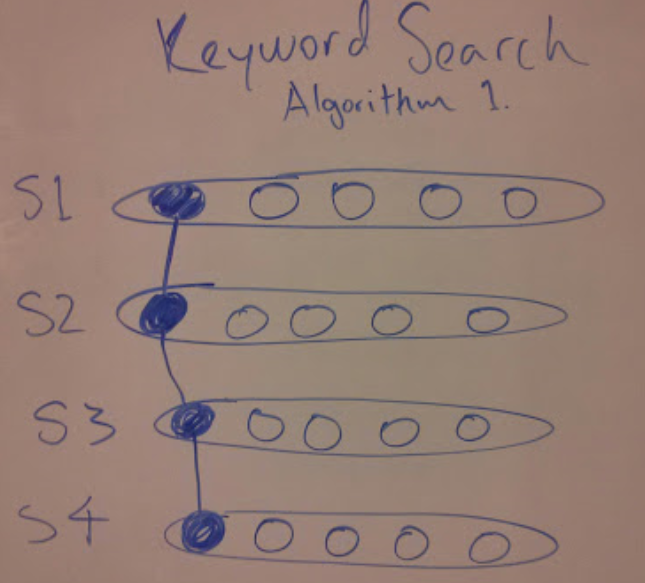
\includegraphics[height=2in, width=4in]{Images/KeywordSearchAlg1.png}
\caption{A visualization of keyword selection using search criterion 1. Here, each oval denotes a sentence, each circle a word or embedding. Embeddings have been sorted by corresponding search criterion 1 values, minimum values denoted by solid blue circles. The search space here is highly constrained but leads to the minimum search criterion 1 value of $\gamma^{min}$.}
\end{figure}

By allowing our selection algorithm to reach a value of $\hat{\gamma} > \gamma^{min}$, we relax the search space boundaries and are able to select keywords from a bigger embedding subset, while also reducing the search space from the original unconstrained search space i.e. ignoring "common" words.

We now introduce the \textit{\textbf{budget}} parameter $\lambda$. This weight parameter controls how much more cosine similarity we are willing to add into our model i.e. deviate from $\gamma_{i}^{min}$ in order to increase our search space from the highly constrained search space, while avoiding the original entire search space found with $\gamma^{max}$. We thus define a new search criterion 1 metric that leads to a reduced search space from the original search space but allows more exploration room than $\gamma_{i}^{min}$: \[\hat{\gamma_{i}} = \gamma_{i}^{min} + \lambda x\]
In this work we consider $x = \gamma_{i}^{max}-\gamma_{i}^{min}$.

We now present an algorithm for determining the sentence search space boundary given a search criterion 1 value $\hat{\gamma_{i}}$. For notation convenience, we denote $\bm{\vec{\bar{c_i}}}$ as the sorted form of $\bm{\vec{c_i}}$:

\begin{algorithm}[H]
\caption{Compute Search Space Boundaries}
\begin{algorithmic}[1]
\Procedure{ComputeSearchSpaceBoundaries}{$\lambda,\bm{\vec{\bar{c_1}}}, ..., \bm{\vec{\bar{c_n}}}$}
\For {$i$ = 1 to $n$}
\State$ \gamma_{i}^{min} = \bm{\vec{\bar{c_i}}}[1]$
\State$ \gamma_{i}^{max} = \bm{\vec{\bar{c_i}}}[| \bm{\vec{\bar{c_i}}}|]$
\State$ \hat{\gamma_{i}} = \gamma_{i}^{min} + \lambda(\gamma_{i}^{max} - \gamma_{i}^{min})$

\State $idx_i = \textit{ComputeSearchSpaceBoundaries}(\gamma_{i}^{min}, \hat{\gamma_{i}}, \bm{\vec{\bar{c_i}}})$
 \EndFor




\Return $\bm{\vec{idx}} = (idx_1, ..., idx_n)$
\EndProcedure
\end{algorithmic}
\end{algorithm}

\begin{algorithm}[H]
\caption{Compute Search Stop Index}\label{euclid}
\begin{algorithmic}[1]
\Procedure{ComputeSearchSpaceBoundaries}{$\gamma_{i}^{min}, \hat{\gamma_{i}}, \bm{\vec{\bar{c_i}}}$}

\State $idx_i = 1$

\State $\gamma\prime \gets \gamma_{i}^{min}$
\While{$ \gamma\prime \leq \hat{\gamma_{i}}$}
\State $idx_i \gets idx_i + 1$
\State $\gamma\prime \gets \gamma\prime + \bm{\vec{\bar{c_i}}}[idx_i]$


\EndWhile
\\
\Return $idx_i$
\EndProcedure
\end{algorithmic}
\end{algorithm}

Using Algorithm 3, we compute the search space boundary defined by the returned index vector $\bm{\vec{idx}} = (idx_i, ..., idx_n)$. After the algorithm completes, for sentence $s_i$,  we are allowed to search from index $1$ to $idx_i$.
The variable $\gamma\prime$ is initialized to $\gamma^{min}$, and incremented until we reach a value of at most $\hat{\gamma}$. Hence, $\hat{\gamma}$ determines the search space boundary shape.

\begin{figure}[H]
\centering
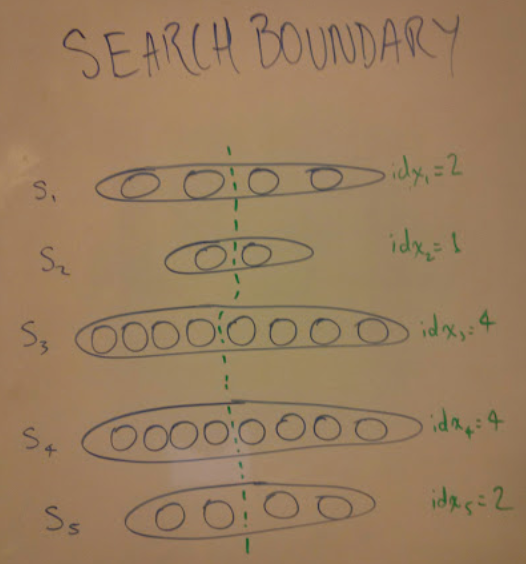
\includegraphics[height=3in, width=4in]{Images/SearchBoundary.png}
\caption{A visualization of five sentences, with their embeddings sorted by increasing search criterion 1. This search space is bounded by $\hat{\gamma}$, relaxing the boundary imposed by $\gamma^{min}$, while reducing the size of the original search space, as denoted by the illustration. Here an ideal example is shown, where the boundary parameter $\hat{\gamma}$ created a 50 percent search space reduction. The search boundary is denoted by a dashed green line, and defined by the index number corresponding to all sentences, shown in the far right.}
\end{figure}


\section{Keyword Selection Algorithms}
Having introduced an algorithm for creating a search space boundary based on \textit{search criterion 1}, we now introduce keyword extraction algorithms based on \textit{search criterion 2} on the reduced search space determined using algorithm 4. First we will develop on a greedy algorithm, choosing keywords one step at a time and choosing the best choice at each stage. We then develop on a keyword search fomulated as a minimization of an objective function based on search criterion 1 and 2.

\subsection{Linear Information Propagation (Greedy)}
Given a set of sentences $\bm{S}$, we assume that the contents of the $i+1$th sentence are directly influenced by the contents of the $i$th sentence. Furthermore, we assume that a set of sentences under the LIP model has a \textit{\textit{local topic}}, and can be encapsulated as a set of keywords, one for each sentence.

\begin{figure}[H]
\centering
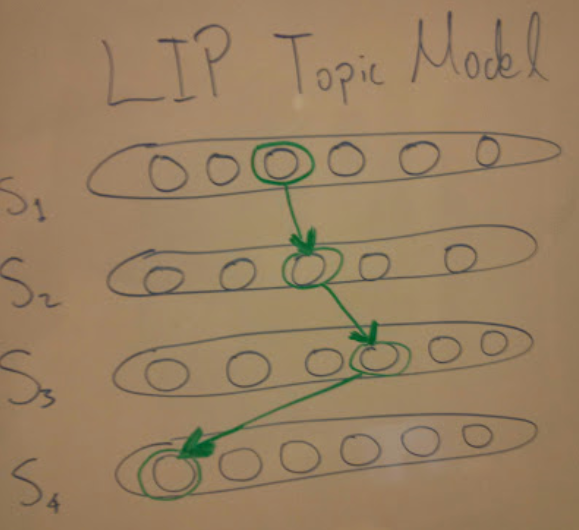
\includegraphics[height=3in, width=4in]{Images/LIPTopic.png}
\caption{A visualization of the LIP Topic model. Given an ordered set of sentences $S$, i.e. text, the model assumes that the contents of a sentence depends on the contents of the previous sentence. Furthermore, a \textit{local topic} is assumed occur throughout the contents of the text, and is encapsulated by a set of keywords, one for each sentence. Here, the topic words and flow of information are denoted by green circles and arrows respectively.}
\end{figure}

\begin{figure}[H]
\centering
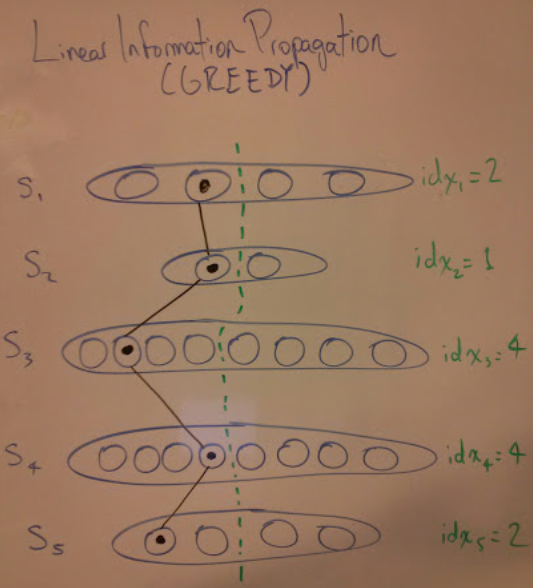
\includegraphics[height=3in, width=4in]{Images/LIPGreedy.png}
\caption{A visualization of the Greedy LIP algorithm. Based on the reduced search space, we find the word in the $i+1$th sentence such that we maximize the cosine similarity with the chosen word in the the $i$th sentence. The chosen keywords are denoted by circles with black dots. At each step, a greedy selection is made, considering only the $i$th and $i+1$th sentences and \textit{search criterion 2}.}
\end{figure}


\begin{algorithm}[H]
\caption{LIP (Greedy) Keyword Extraction}\label{euclid}
\begin{algorithmic}[1]
\Procedure{LIPGreedyKeywordExtraction}{$(\bm{\vec{\bar{c_1}}}, ..., \bm{\vec{\bar{c_n}}}), \bm{\vec{idx}}$}
\For {$i$ = 1 to $n$}
\State $sel_i \gets 0$
 \EndFor
\State $d \gets 0$
\State $sim \gets 0$

\For{$i$ = 1 to $\bm{\vec{idx[1]}}$}
        \For{$j$ = 1 to $\bm{\vec{idx[2]}}$}
            \State$sim \gets\bm{\vec{\bar{c_1[i]}}} \cdot \bm{\vec{\bar{c_2[j]}}}$
          \If{$sim \textgreater d$}
              \State $d \gets sim$
              \State$ sel_1 \gets i$
              \State $ sel_2 \gets j$
         \EndIf
        \EndFor
\EndFor

\For{ $k$ = 3 to $n$}
    \State $d \gets 0$
    \For {$i$ = 1 to $\bm{\vec{idx[k]}}$}
        \State$sim \gets \bm{\vec{\bar{c_{k-1}[sel_{k-1}]}}} \cdot \bm{\vec{\bar{c_{k}[sel_{i}]}}}$
        \If{$sim \textgreater d$}
              \State$d \gets sim$
              \State$sel_k \gets i$
        \EndIf
    \EndFor
\EndFor
\Return $\bm{\vec{sel}} = (sel_1, ..., sel_n)$

\EndProcedure
\end{algorithmic}
\end{algorithm}


\subsection{Objective Function Search}
Search criterion 2 seeks to maximize \textit{over-paragraph} cosine similarity i.e. how similar the selected terms are to each other. Search criterion 1 on the other hand seeks terms that minimize how similar they are to their \textit{neighbor terms} i.e. minimize \textit{within-sentence} cosine similarity. These two search criteria are seemengly contradictory. The first criterion tries to minimize cosine similarity, while the second one tries to maximize it. It is when the two terms are combined as an objective function when they provide a more solid foundation for keyword extraction based on semantic relations. For ease of notation, we always denote a paragraph i.e. our input text as $S$ and overload indexing operations in a way similar to matrix indexing. $S_{i}$ denotes the $i$th sentence, and $S_{i,j}$ denotes the $j$th word in the $i$th sentence. We thus define our search objective function as
\[J = \Gamma - \Delta\]

where
\[\Gamma(i,j) = \sum\limits_{j} [S_{i}^ T \times S_{i}]_{i,j}\]



\section{Topic Extraction}
\subsection{Baseline: Simple Voting Scheme}
\subsection{K-Means Clustering}
\section{Performance Evaluation}
\subsection{Keyword Evaluation: Relevance Measure}
\subsection{Keyword Evaluation: 0-1 Loss}
test
\subsection{Keyword Evaluation: Mean Squared Error}
\section{Application: Automatic Keyword Detection in Research Papers}
\end{document}
